\section{LPPL模型的求解}
\subsection*{模型一般的求解方式}
\begin{frame}[t]{一般求解方式}
    假设我们已经已经获取到数据,$\set{(t_i,p_i)}{\forall i\in[1,n]\cap\zz}$。其中数据对$(t_i,p_i)$指的是,在时间$t_i$下,价格为$p_i$。
    
    首先,我们来解决线性参数$A$,$B$,$C_1$与$C_2$的求解。为突出线性部分,我们令:
    \begin{equation*}
        \begin{cases}
            f_i(t_c,m)        &= (t_c-t_i)^m \\
            g_i(t_c,m,\omega) &= (t_c-t_i)^m\cos\left[\omega\ln(t_c-t_i)\right] \\
            h_i(t_c,m,\omega) &= (t_c-t_i)^m\sin\left[\omega\ln(t_c-t_i)\right] \\
        \end{cases}
    \end{equation*}
    将上是代入LPPL模型中有:
    \begin{equation*}
        \begin{pmatrix}
            1      & f_1    & g_1    & h_1    \\
            1      & f_2    & g_2    & h_2    \\
            \vdots & \vdots & \vdots & \vdots \\
            1      & f_n    & g_n    & h_n    \\
        \end{pmatrix}
        \begin{pmatrix}
            A \\ B \\ C_1 \\ C_2
        \end{pmatrix}
        =
        \begin{pmatrix}
            \ln(p_1) \\ \ln(p_2) \\ \vdots \\ \ln(p_n) \\
        \end{pmatrix}
    \end{equation*}
\end{frame}

\begin{frame}[t]{一般求解方式}
    简记为$\matx\vecb = \vecy$。于是有:
    \begin{align*}
        \hat{\vecb} &= \left(\matx^T\matx\right)^{-1}\matx^T\vecy \\
                    &=
        \begin{pmatrix}
            \sum 1   & \sum f_i    & \sum g_i    & \sum h_i    \\
            \sum f_i & \sum f_i^2  & \sum f_ig_i & \sum f_ih_i \\
            \sum g_i & \sum f_ig_i & \sum g_i^2  & \sum g_ih_i \\
            \sum h_i & \sum f_ih_i & \sum g_ih_i & \sum h_i^2  \\
        \end{pmatrix}^{-1}
        \begin{pmatrix}
            \sum \ln(p_i)    \\
            \sum f_i\ln(p_i) \\
            \sum g_i\ln(p_i) \\
            \sum h_i\ln(p_i) \\
        \end{pmatrix}
    \end{align*}
\end{frame}


\begin{frame}[t]{一般求解方式}
    根据克莱姆法则可知四阶矩阵的逆表达式十分繁杂,所以只能采用数值方式进行求解LPPL模型。残差平方和可以表示为
    \begin{equation*}
        Res = \norm{\vecy-\matx\hat{\vecb}}_2^2.
    \end{equation*}
    在这一步,就找到了使用优化算法的函数,将$t_c$,$m$与$\omega$代入后即可使用常规的优化算法来求解。而由于LPPL模型的特殊性,其优化算法得出来的解可能对初始值的依赖很大。于是取不同的初值点进行优化,取使$Res$最小的优化解。
\end{frame}


\begin{frame}[t]{模型求解的实例:SSEC}
    \begin{figure}[H]
        \subcaptionbox{}{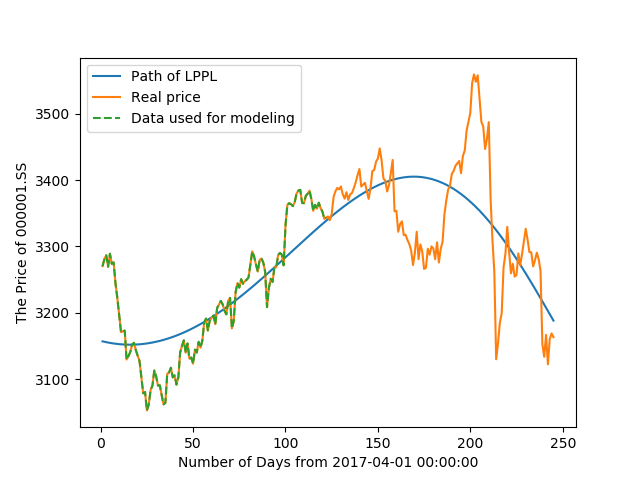
\includegraphics[width=.45\textwidth]{figures/000001SS.png}}
        \subcaptionbox{}{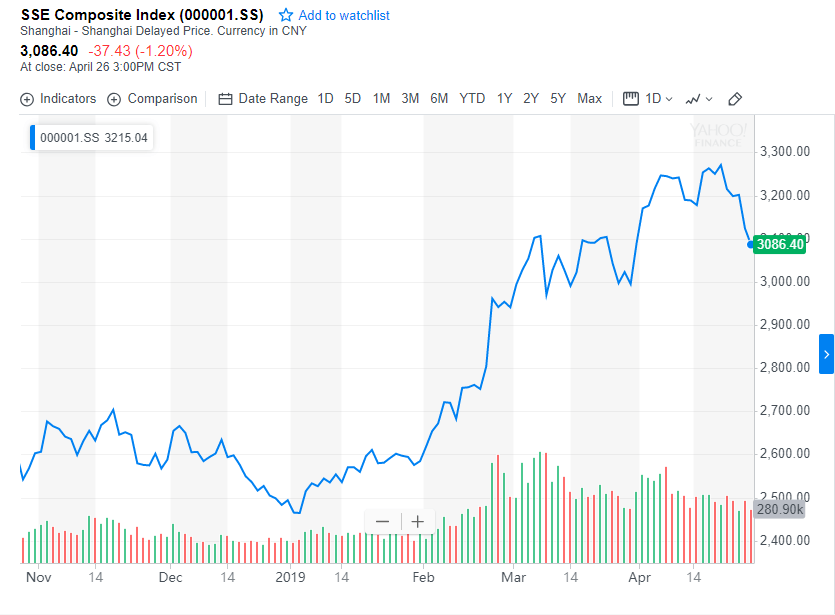
\includegraphics[width=.45\textwidth]{figures/finance-yahoo-1.png}}
    \end{figure}
    \begin{table}[H]
        \begin{tabular}{@{}lccccccc@{}}
        \toprule
                               & $m$  & $\omega$ & $t_c$  & $A$              & $B$             & $C_1$      & $C_2$         \\ \midrule
        000001.SS & 1.00 & 5.64     & 448.48 & 0.00 & 0.00 & 0.00 & -0.00 \\ \bottomrule
        \end{tabular}
        \caption{LPPL模型的一般求解结果}\label{T:Solution-1}
    \end{table}
\end{frame}

\begin{frame}[t]{模型求解的实例:DJIA}
    \begin{figure}[H]
        \subcaptionbox{}{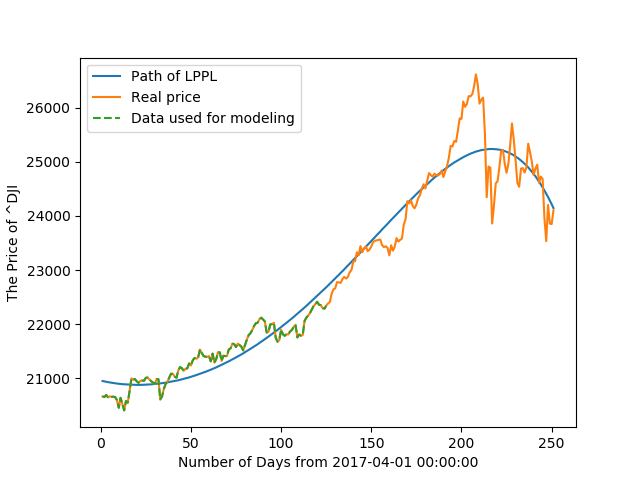
\includegraphics[width=.45\textwidth]{figures/^DJI.png}}
        \subcaptionbox{}{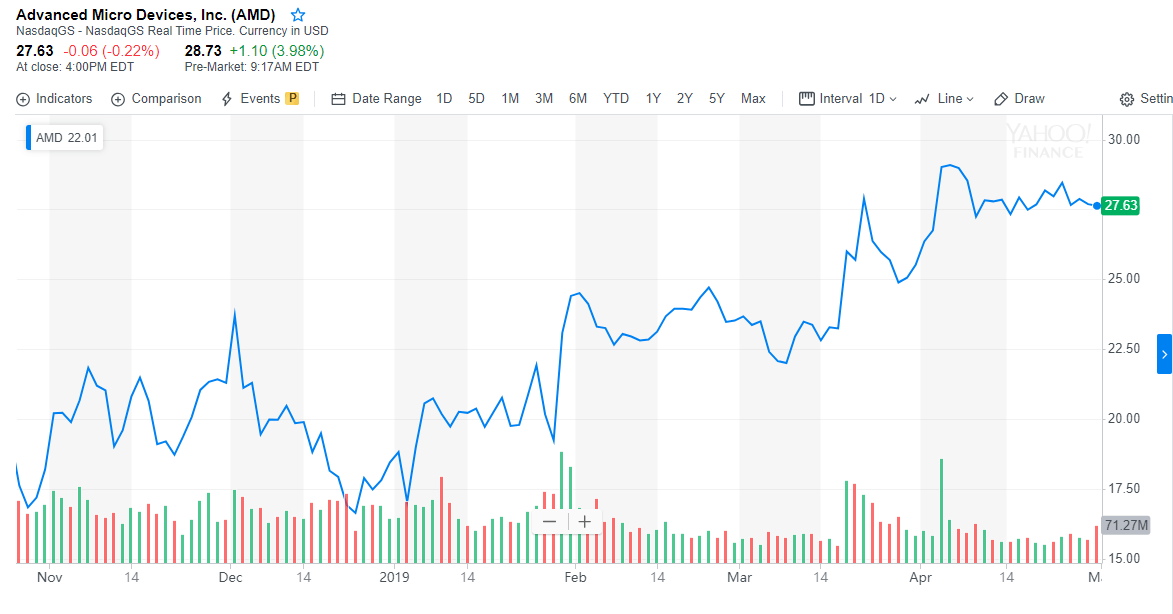
\includegraphics[width=.45\textwidth]{figures/finance-yahoo-2.png}}
    \end{figure}
    \begin{table}[H]
        \begin{tabular}{@{}lccccccc@{}}
        \toprule
                               & $m$  & $\omega$ & $t_c$  & $A$              & $B$             & $C_1$      & $C_2$         \\ \midrule
        \textasciicircum{}DJI  & 0.00 & 0.05     & 458.08 & -4.7e11 & 4.7e11 & 2.4e4   & -7.9e4     \\ \bottomrule
        \end{tabular}
        \caption{LPPL模型的一般求解结果}\label{T:Solution-2}
    \end{table}
\end{frame}

\begin{frame}[t]{模型求解的实例:SPX}
    \begin{figure}[H]
        \subcaptionbox{}{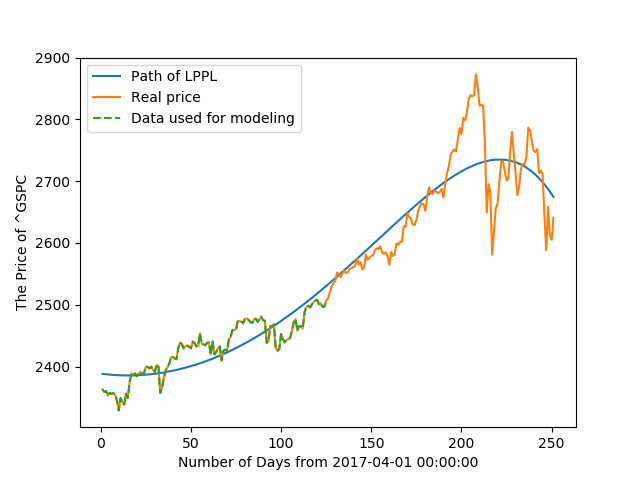
\includegraphics[width=.45\textwidth]{figures/^GSPC.png}}
        \subcaptionbox{}{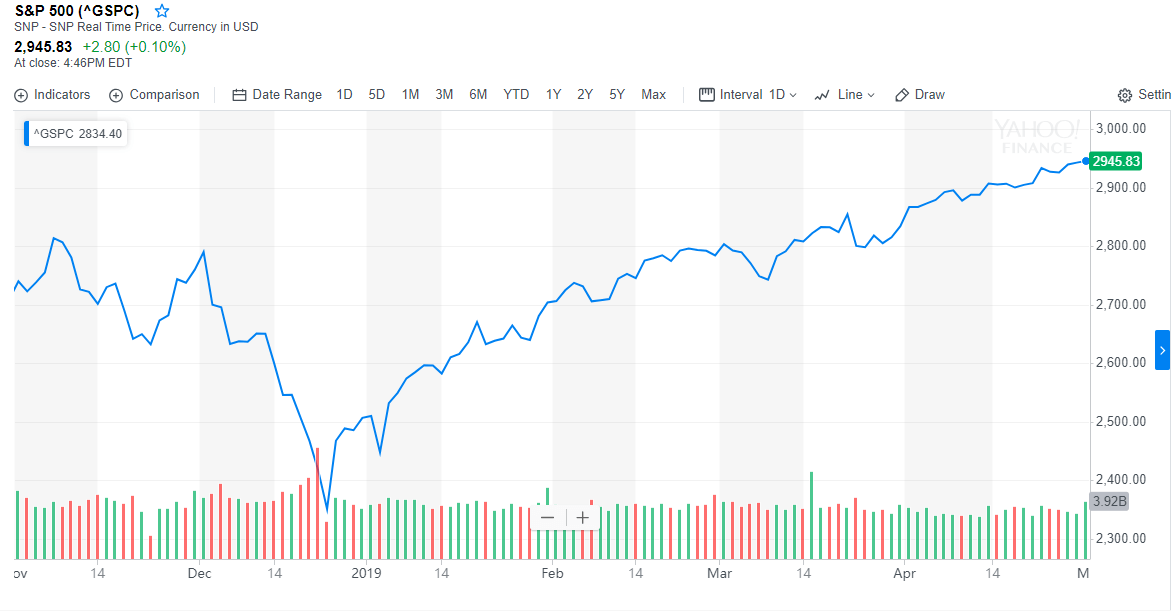
\includegraphics[width=.45\textwidth]{figures/finance-yahoo-3.png}}
    \end{figure}
    \begin{table}[H]
        \begin{tabular}{@{}lccccccc@{}}
        \toprule
                               & $m$  & $\omega$ & $t_c$  & $A$              & $B$             & $C_1$      & $C_2$         \\ \midrule
        \textasciicircum{}GSPC & 0.00 & 0.00     & 451.00 & -2.4e11 & 2.4e11 & 5.3e6 & -4.3e8 \\ \bottomrule
        \end{tabular}
        \caption{LPPL模型的一般求解结果}\label{T:Solution-3}
    \end{table}
\end{frame}
